\chapter{MÉTODO DE COMPRESIÓN PROPUESTO}\label{chap:clustering}
\vskip 3.0ex

En esta sección se procede a desarrollar el algoritmo de compresión de grafos dispersos, usando estructuras compactas y aprovechando la redundancia de vértices del grafo en sus cliques maximales.

Esto consta de tres etapas. La primera consta de listar todos los cliques maximales del grafo. Luego se define una heurística eficiente para agrupar o particionar los cliques, aprovechando la superposición entre ellos. Finalmente se define una estructura compacta basada en secuencias para almacenar las particiones. 


\section{Detección de cliques maximales}

La representación del grafo mediante su grafo de cliques (ver Definición \ref{def:cliqueGraph}) conlleva un problema, listar los cliques maximales de un grafo. Enumerarlos todos es un problema complejo desde un punto de vista teórico y práctico. 

Eppstein et. al. \cite{eppstein2010listing, eppstein2011listing} proponen un algoritmo rápido para listar cliques maximales de grafos poco densos. La complejidad de su algoritmo es $O(dn3^{d/3})$ en tiempo y $O(n+m)$ en espacio, siendo $d$ el índice de \textit{degeneracy}, $n$ la cantidad de vértices, y $m$ la cantidad de aristas del grafo (ver Sección~\ref{sec:Cliques}).

Este algoritmo está disponible en el repositorio \textbf{Quick Cliques}\footnote{\url{https://github.com/darrenstrash/quick-cliques}}, implementado por los mismos autores. Luego, el problema se concentra en encontrar un método eficiente para dividir en particiones el grafo de cliques, que permita tanto ahorrar espacio como responder consultas sobre el grafo de manera rápida.

Con el listado de cliques maximales, se puede obtener el grafo de cliques del grafo, el cual se define a continuación. 

\begin{definition} 
	\label{def:cliqueGraph}
	Gafo de cliques
	
	Dado un grafo $G = (V, E)$ y $\mathcal{C} = \{c_{1}, c_{2}, ..., c_{N} \}$ el conjunto de tamaño $N$ de cliques maximales que cubren $G$, se tiene $CG_{\mathcal{C}} = (V_{\mathcal{C}}, E_{\mathcal{C}})$ un grafo de cliques donde:
	
	\begin{enumerate}
		\item $V_{\mathcal{C}} = \mathcal{C}$
		\item $\forall c, c' \in \mathcal{C}, (c, c') \in E_{\mathcal{C}} \Longleftrightarrow c \cap c' \neq \varnothing$
	\end{enumerate}
\end{definition}

En la Figura \ref{fig:gafoEj} (a) se muestra un grafo no dirigido de ejemplo, en la Figura \ref{fig:gafoEj} (b) su listado de cliques maximales, y en la Figura \ref{fig:gafoEj} (c) el grafo de cliques resultante.


\begin{figure}
    	\centering
    	\begin{minipage}{0.4\textwidth}
    		\centering
    		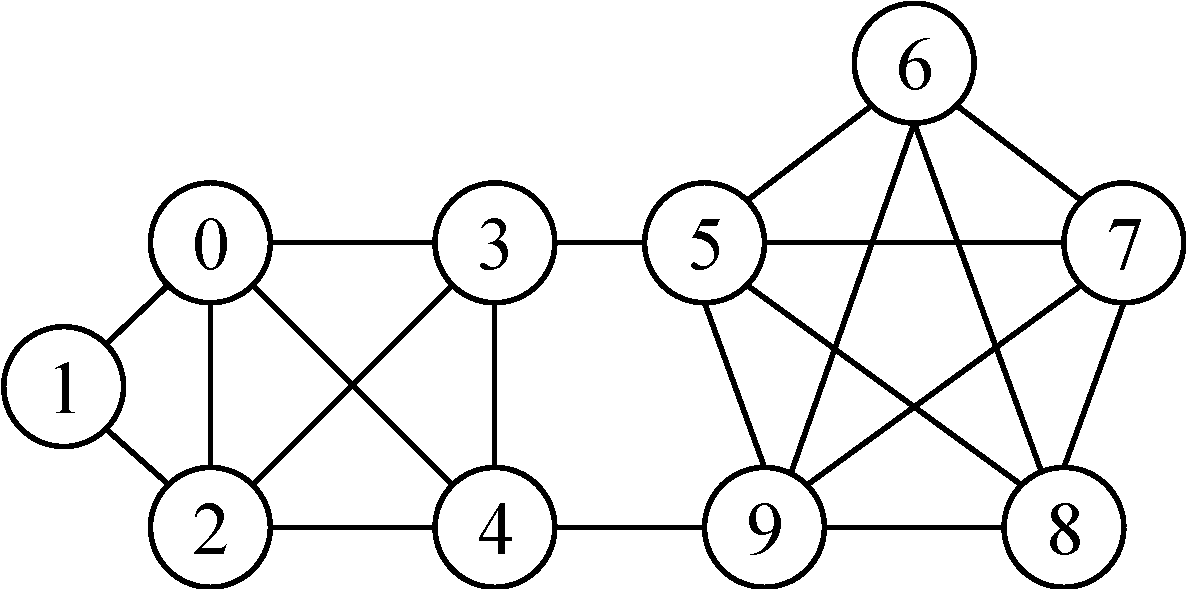
\includegraphics[width=1\linewidth,clip=true]{img/graphs-Graph2.pdf}
    		(a)
    	\end{minipage}
    	\begin{minipage}{0.4\textwidth}
    		\centering
    		\[
	\begin{aligned}[t]
		C_{0} &: 0, 1, 2 \\
		C_{1} &: 0, 2, 3, 4 \\
		C_{2} &: 3, 5 \\
		C_{3} &: 5, 6, 7, 8, 9 \\
		C_{4} &: 4, 9
	\end{aligned}
\]

    		(b)
    	\end{minipage}
    	\begin{minipage}{0.15\textwidth}
    		\centering
    		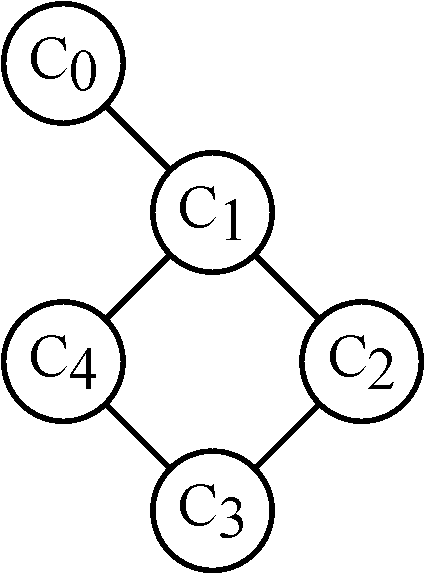
\includegraphics[width=1\linewidth,clip=true]{img/graphs-Cliques2.pdf}
    		(c)
    	\end{minipage}
    \caption{(a) Grafo no dirigido. (b) Lista de cliques maximales. (c) Grafo de cliques.}
    \label{fig:gafoEj}
\end{figure}




\section{Particionamento del grafo de cliques}

Teniendo el grafo de cliques maximales, es necesario definir una heurística que permita agruparlos en particiones de manera eficiente, pensando tanto en el espacio que ocuparán las secuencias comprimidas como en tiempos de acceso secuencial y aleatorio.

Se desean encontrar particiones del grafo de cliques que exploten dicha redundancia de vértices en los cliques maximales, y permita agrupar en una misma partición a cliques que tengan una cantidad razonable de vértices en común, y los que no la tengan queden separados en otras particiones. El problema de encontrar particiones de cliques se define a continuación.

\begin{problem}
	\label{def:findPartitions}
	Encontrar particiones de cliques para el grafo de cliques $CG_{\mathcal{C}}$.
	
	Dado un grafo de cliques $CG_{\mathcal{C}} = (V_{\mathcal{C}}, E_{\mathcal{C}})$, encontrar un set de particiones de cliques $\mathcal{C}\mathcal{P} = \{cp_{1}, cp_{2}, ..., cp_{M}\}$ de $CG_{\mathcal{C}}(V_{\mathcal{C}}, E_{\mathcal{C}})$ con $M \geq 1$, tal que
	\begin{enumerate}
		%\item $\bigcup_{i \in \mathcal{C}\mathcal{P}} cp_{i} = CG_{i}$ \label{item:particiones1}
		\item $\bigcup\limits_{i = 1}^{M} cp_{i} = CG_{\mathcal{C}}$ \label{item:particiones1}
		\item $cp_{i} \cap cp_{j} = \varnothing$ para $i \neq j$ \label{item:particiones2}
		\item cualquier $cp_{i} \in \mathcal{C}\mathcal{P}$ es un subgrafo de $CG_{\mathcal{C}}(V_{\mathcal{C}}, E_{\mathcal{C}})$ inducido por el subset de vértices en $cp_{i}$ \label{item:particiones3}
	\end{enumerate}
	
\end{problem}

Esto indica que cada partición es un subgrafo del grafo de cliques maximales del grafo $G(V,E)$. El punto~\ref{item:particiones2} es importante, ya que prohíbe que un clique se repita en una partición, no así un subset de vértices de grafo $G(V,E)$ que sí puede estar en varias particiones a la vez.

%Se presentan tres alternativas. La primera consta en conocer con qué frecuencia aparece cada vértice en todos los cliques, y agruparlos según los nodos más frecuentes. La segunda consta en evaluar por nodo, cuántos nodos están conectados a él por clique, para luego agruparlos según los nodos más conectados. Finalmente, se agrupa mediante la razón entre ambos métodos.

A continuación se plantea una heurística que, basada en el listado de cliques maximales $\mathcal{C} = \{c_{1}, c_{2}, ..., c_{N} \}$ y funciones de ranking, genere el particionamiento del grafo de cliques sin necesidad de generar dicho grafo.


\section{Algoritmo de particionamiento o clustering} \label{sec:PartitionAlgoritms}

En esta sección se procede a describir el algoritmo para generar las particiones del grafo de cliques. Para ello, en la Definición~\ref{def:rankingFunctions} se define una función de ranking, que valoriza cada vértice según ciertas características. También se detallan ciertas funciones de ranking basadas en la cantidad y tamaño de los cliques maximales donde un vértice se encuentre.

\begin{definition} 
	\label{def:rankingFunctions}
	Función de ranking
	
	Dado un grafo $G = (V, E)$ y $\mathcal{C} = \{c_{1}, c_{2}, ..., c_{N} \}$ el conjunto de tamaño $N$ de cliques maximales que cubren $G$, una función de ranking es una función $r: V \rightarrow \mathbb{R}^{+}$ que retorna un valor de puntuación para cada vértice $v \in V$.
\end{definition}

La heurística de clustering se describe en el Algoritmo~\ref{alg:clustering}. La salida del cálculo de ranking son los arreglos $D$ y $R$ (Algoritmo~\ref{alg:clustering} línea \ref{alg:clustering:rankarray}), donde $D$ contiene los índices de los cliques donde cada vértice del grafo $G$ participan, y $R$ contiene el valor de puntuación para cada vértice en $G$. La complejidad del algoritmo de cálculo de ranking se compone primero por pasar por todos los vértices en $G$ en el conjunto de cliques maximales $\mathcal{C}$, y luego ordenar $R$ de mayor a menor. La complejidad total del algoritmo es de $O(L \log L)$, donde $L=\sum_{c_i \in \mathcal{C}}|c_{i}|$.

Luego se crea un arreglo de bits $Z$ de largo $N = |\mathcal{C}|$ iniciando cada bit en cero, el cual servirá para mantener revisado si un clique ya fue incluido o no en una partición. Se recorre el arreglo $R$ y por cada vértice $u$, se obtienen los índices de los cliques donde $u$ participa según $D[u]$ y se añaden el índice $id$ de cada clique a la partición pertinente ($cpid$) solo si $Z[id] = 0$. Si el índice $id$ fue exitosamente agregado, se cambia el valor de $Z[id] = 1$. Si la partición $cpid$ contiene al menos un índice de clique, la partición es agregada a la colección $\mathcal{C}\mathcal{P}$, y se continúa procesando vértices en $R$. La complejidad del algoritmo para este paso es de $O(N+V)$. Finalmente, el algoritmo retorna la colección de particiones $\mathcal{C}\mathcal{P}$, donde cada partición contiene un set de los índices de cliques que las componen.

\begin{algorithm}
\caption{Algoritmo de particionamiento del grafo de cliques.}
\label{alg:clustering}
\begin{algorithmic}[1]
\REQUIRE $\mathcal{C}$ maximal clique collection ($N=|\mathcal{C}|$), ranking function $r(u)$
\ENSURE Returns clique-graph partition collection $\mathcal{C}\mathcal{P}$
\STATE $(D,R) \leftarrow computeRanking(r,\mathcal{C})$ (array $D$ y $R$, $\forall u \in V$ ) \label{alg:clustering:rankarray} 
\STATE Initialize bit array $Z$ of size $N$ and set each bit to 0
\FOR {$u \in R$}
    \STATE $cpid \leftarrow \emptyset$
     \FOR {$id \in D[u]$ and $D[u]=0$} 
          \STATE $Z[id] \leftarrow 1$
          \STATE $cpid \leftarrow cpid \cup \{id\}$
    \ENDFOR
    \IF {$cpid \neq  \emptyset$}
      \STATE $\mathcal{C}\mathcal{P} \leftarrow \mathcal{C}\mathcal{P} : cpid$
    \ENDIF 
 \ENDFOR
\RETURN $\mathcal{C}\mathcal{P}$
\end{algorithmic}
\end{algorithm}


Las funciones de ranking (Definición~\ref{def:rankingFunctions}) que se proponen toman en cuenta la cantidad y el tamaño de los cliques donde participa cada vértice del grafo $G(V, E)$. Primero se define el conjunto $C(u)$ para cada vértice $u \in V$ como $C(u) = \{c \in \mathcal{C}|u \in c\}$, luego las funciones de rankings son las siguientes:

\begin{align}
	r_{f}(u) &= |C(u)| \label{eq:rankFunF}  \\ 
	r_{c}(u) &= \sum_{c \in C(u)}|c| \label{eq:rankFunC} \\ 
	r_{r}(u) &= \frac{r_{c}(u)}{r_{f}(u)} \label{eq:rankFunR}
\end{align}


La función $r_{f}(u)$ (ec. \ref{eq:rankFunF}) indica en cuántos cliques está presente el vértice $u$, la función $r_{c}(u)$ (ec. \ref{eq:rankFunC}) entrega la suma del tamaño de los cliques donde está presente el vértice $u$, y la función $r_{r}(u)$ (ec. \ref{eq:rankFunR}) es la razón entre $r_{c}(u)$ y $r_{f}(u)$. En la Figura~\ref{fig:sequences} se muestra el resultado de las funciones de ranking para el caso ejemplo, y las particiones de cliques resultantes para cada una.

\begin{figure}
    \centering

    \begin{minipage}{\textwidth}
    	\centering
    	\begin{tabular}{c|c|c|c|c|c|c|c|c|c|c|}
	\cline{2-11}
	$u \in G$ & 0 & 1 & 2 & 3 & 4 & 5 & 6 & 7 & 8 & 9 \\
	\cline{2-11}
	$R_{rf}$ & 2,0 & 1,0 & 2,0 & 2,0 & 2,0 & 1,0 & 1,0 & 1,0 & 1,0 & 2,0 \\
	\cline{2-11}
	$R_{rc}$ & 7,0 & 3,0 & 7,0 & 6,0 & 6,0 & 7,0 & 5,0 & 5,0 & 5,0 & 7,0 \\
	\cline{2-11}
	$R_{rr}$ & 3,5 & 3,0 & 3,5 & 3,0 & 3,0 & 3,5 & 5,0 & 5,0 & 5,0 & 3,5 \\
    \cline{2-11}
\end{tabular}

    	
    	(a)
    \end{minipage}

    \hfill\vline\hfill
    
    \begin{minipage}{\textwidth}
    	\centering
    	\begin{tabular}{c|c|c|c|c|}
	\cline{2-5}
	$\mathcal{C}\mathcal{P}_{rf}$ & $C_{0} \quad C_{1}$ & $C_{2}$ & $C_{4}$ & $C_{3}$ \\
	\cline{2-5}
	$\mathcal{C}\mathcal{P}_{rc}$ & $C_{0} \quad C_{1}$ & $C_{2} \quad C_{3}$ & $C_{4}$ \\
	\cline{2-5}
	$\mathcal{C}\mathcal{P}_{rr}$ & $C_{3}$ & $C_{0} \quad C_{1}$ & $C_{2}$ & $C_{4}$ \\
	\cline{2-5}
\end{tabular}

    	
    	(b)
    \end{minipage}
    
    \caption{Resultados de las funciones de ranking. (a) Puntaje final. (b) Particiones de cliques.}
    \label{fig:sequences}
\end{figure}


\section{Representación en estructuras compactas}

En esta sección se detalla la estructura compacta para representar $G(V, E)$ usando las particiones $\mathcal{C}\mathcal{P}$ obtenida en la Sección~\ref{sec:PartitionAlgoritms}. Se consideran estructuras de datos compactas  basadas en símbolos y secuencias de bits, con soporte para las operaciones de \textit{rank()}, \textit{select()} y \textit{access()}.

\subsection{Secuencias de la representación de las particiones}
La representación de las particiones consta de cuatro elementos, dos secuencias de enteros \textbf{X} e \textbf{Y}, un mapa de bits \textbf{B}, y una secuencia de bytes \textbf{BB}, las cuales se describen a continuación.

\begin{itemize}
	\item La secuencia de enteros \textbf{X} consiste en las listas concatenadas de los vértices presentes en los cliques de cada partición.
	\item El mapa de bits \textbf{B} contiene un bit por cada elemento en \textbf{X} inicializados en cero, indicando el inicio de las particiones con un uno. Además se agrega un bit extra en uno al final de la secuencia para indicar su final.
	\item La secuencia de bytes \textbf{BB} codifica en qué cliques está presente cada vértice, marcando un  $1$ en cada bit de cada byte por clique si el vértice pertenece a ese clique.
	\item La secuencia de enteros \textbf{Y} indica cuántos bytes omitir en \textbf{BB} para acceder rápidamente a la partición deseada.
\end{itemize}

La definición formal de la estructura se presenta en la Definición~\ref{def:sequences}. Se puede observar de la ecuación \ref{eq:bbp} que $BB_{p} \in BB$ es una matriz de bytes, donde cada fila representa un vértice $u$ en $X_{p} \in X$, y las columnas corresponden a los bytes usados por los vértices para marcar los cliques donde participan en la partición. 

También se debe notar el caso especial, cuando un clique maximal queda solo en una partición, no ocupa espacio en su $BB_{p}$ correspondiente. Para poder reconocer estos casos, se agrupan al final de la estructura compacta todas estas particiones, y con esto se puede ahorrar espacio tanto en $BB$ como en $Y$.

\begin{definition} 
	\label{def:sequences}
	Representación compacta del grafo $G(V, E)$. 
	
	Dado $\mathcal{C}\mathcal{P} = \{cp_{0},...,cp_{M-1}\}$, $cp_{p} \in \mathcal{C}\mathcal{P}$, y $cp_{p}=\{c_{0},...,c_{m_{r}-1}\}$. 
	Se especifica $bpu_{p} = \ceil*{\frac{m_{r}-1}{8}}$ como la cantidad de bytes por vértice $u$ en $X_{p}$, y se definen las secuencias $X_{p}$, $B_{p}$, $BB_{p}$, $Y_{p}$ como sigue:
	
	\begin{align}
		X_{p} &= \{u \in c|c \in cp_{p}\} = \{u_{0},...u_{|X_{p}|-1}\} \\
		B_{p} &= 1:0^{|X_{p}|-1} \\
		BB_{p} &= bb[|X_{p}|][bpu_{p}]   \label{eq:bbp} \\
		bb[i][j] &= \begin{cases}
                  \sum_{k=0}^{7} 2^{k}(u_{i} \in c_{8j+k}), & bpu_{p} \neq 0  \\
                  %, & x \in c , x \in X_{p}, c \in OC_{r} \\
                  \emptyset, & otherwise \\
                 \end{cases} \nonumber \\
		Y_{p} &= \begin{cases}
				|X_{p}|\times bpu_{p} + Y_{p-1}, & bpu_{p} \neq 0  \\
				 \emptyset, & otherwise \\
			\end{cases}
	\end{align}
\end{definition}

\textcolor{red}{Cambié la definición de Y, para dejar en claro que si una partición no tiene bytes en BB, tampoco tendrá un Y asociado.}

En la Figura~\ref{fig:compactStructure} se presenta la estructura resultante del ejemplo, usando las particiones $\mathcal{C}\mathcal{P}_{rr}$ reordenadas. Como se puede apreciar, solo la primera partición tiene dos cliques, por tanto será la única que agregue bytes en la secuencia $BB$, codificando la pertenencia de cada clique en un bit del byte, requiriendo entonces solo un byte por vértice en $X$.

La secuencia $X$ se conforma por todos los vértices que conforman los cliques en cada partición, ordenados de menor a mayor. La secuencia $B$ escribe un 1 en cada inicio de una partición más uno extra para indicar el final. Para la secuencia $BB$, los cliques involucrados son $C_{0}: \{0, 1, 2\}$ y $C_{1}: \{0, 2, 3, 4\}$, ambos contienen los vértices $0$ y $2$, codificado con sus bytes en $3$, el vértice $1$ solo está presente en $C_{0}$ y se codifica con su respectivo byte en $1$, y los vértices $3$ y $4$ solo participan en $C_{1}$ y sus bytes toman el valor $2$. Finalmente la secuencia $Y$ se inicia con un  5 por la cantidad de cliques presentes en la primera partición, y como las siguientes solo tienen un clique, no se agregan más enteros.

\begin{figure}
	\centering
	\begin{minipage}{0.45\textwidth}
		\centering
		\begin{tabular}{c|c|c|c|c|}
	\cline{2-5}
	$\mathcal{C}\mathcal{P}_{rr}$ &  $C_{0} \quad C_{1}$ & $C_{3}$ & $C_{2}$ & $C_{4}$ \\
	\cline{2-5}
\end{tabular}

	
		(a)
	\end{minipage}
	\begin{minipage}{0.45\textwidth}
		\centering
		\begin{tabular}{c|c|c|c|c|c|c|c|c|c|c|c|c|c|c|c|}
	\cline{2-15}
	$X$: & 0 & 1 & 2 & 3 & 4 & 5 & 6 & 7 & 8 & 9 & 3 & 5 & 4 & 9 \\
	\cline{2-16}
	$B$: & 1 & 0 & 0 & 0 & 0 & 1 & 0 & 0 & 0 & 0 & 1 & 0 & 1 & 0 & 1 \\
	\cline{2-16}
	$BB$: & 3 & 1 & 3 & 2 & 2 \\
	\cline{2-6}
	$Y$: & 0 & 5 \\
	\cline{2-3}
\end{tabular}

		
		(b)
	\end{minipage}
	
	\caption{Ejemplo de reordenamiento y estructura compacta. (a) $\mathcal{C}\mathcal{P}_{rr}$ reordenado. (b) Estructura compacta reordenada.}
	\label{fig:compactStructure}
\end{figure}



\subsection{Algoritmos de consulta}
A continuación se presentan los algoritmos de consulta que soporta la estructura compacta. El Algoritmo~\ref{alg:sequential} reconstruye el grafo $G(V, E)$ recorriendo de manera secuencial la estructura compacta. El Algoritmo~\ref{alg:neighbors} recupera el listado de vecinos para un vértice cualquiera $u$ del grafo $G(V, E)$. El Algoritmo \ref{alg:twonodes} revisa si dos vértices son vecinos. El Algoritmo~\ref{alg:cliques} recupera el listado de cliques maximales $\mathcal{C}$ del grafo $G(V, E)$.

El algoritmo secuencial (Algoritmo~\ref{alg:sequential}) consiste en recorrer secuencialmente la estructura compacta, revisando los vecinos de cada partición. Si una partición contiene un solo clique entonces todos los vértices asociados son vecinos. Si contiene más de un clique, para cada vértice en $X$ se comparan sus bytes asociados en $BB$ con todos los demás, y si el resultado es distinto de cero, son vecinos. La cantidad de cliques se determina rápidamente al comparar el valor de la secuencia $Y$ de cada partición con la anterior; si es el mismo valor significa que hay un solo clique, si cambió es que hay más de uno.

Para esto, primero se obtiene la cantidad $P$ de particiones, contando la cantidad de unos en la secuencia $B$. Para cada una de ellas, se obtiene el índice del inicio ($s$) y final ($e$) de la partición en $B$. Luego se calcula en $bpu_{p}$ la cantidad de bytes por vértice en la secuencia $X$, y se copia el listado de vértices de la partición actual a RAM para un rápido acceso. Por cada vértice, se revisan los vértices restantes; si la cantidad de bytes por vértice es cero, se agregan todos los pares de vértices a la reconstrucción del grafo. De lo contrario, se comparan todos los bytes por vértice correspondientes, y si dicha comparación da algo distinto a cero, se agrega esa arista a ambos vértices involucrados, y se continúa con el siguiente vértice. Cuando se revisan todas las combinaciones de pares de vértices posibles, se prosigue con la partición siguiente. Finalmente retorna el grafo completo $G$.  La complejidad de este algoritmo es $O(P_{0} \cdot N^{2})$ cuando $bpu_{p}$ es igual a cero, de lo contrario $O(P_{1} \cdot N^{2} \cdot bpu_{p})$, siendo $P_{0}$ el número de particiones con cero bytes por vértice, $P_{1}$ las particiones que sí tienen bytes por vértice, y $N$ el largo de las particiones.

El algoritmo para encontrar vecinos de vértices aleatorios (Algoritmo~\ref{alg:neighbors}) primero detecta las particiones donde participa el vértice $u$ en la secuencia $X$, y luego revisa cada partición detectada. Gracias a las funciones de acceso \textit{rank()}, \textit{select()} y \textit{access()} que soporta la estructura compacta, esta tarea se realiza de manera eficiente.

Primero se cuentan las ocurrencias del vértice $u$, y por cada una se obtiene el inicio y final de las particiones donde está presente, junto con la cantidad de bytes por vértice y la copia a RAM de los vértices que tiene dicha partición. Luego, por cada vértice en la partición y posible vecino, si $bpu_{p}$ es cero se agrega directamente dicho vértice al listado de vecinos de $u$. Si no lo es, se comparan uno a uno los bytes por vértice de $u$ con su posible vecino, y si alguna comparación es distinta de cero, se agrega el vértice en evaluación al listado final y se continúa al siguiente posible. Finalmente retorna el listado de vecinos $N(u)$. La complejidad del algoritmo es $O(M_{0} \cdot N)$ cuando $bpu_{p}$ es igual a cero, y $O(M_{1} \cdot N \cdot bpu_{p})$ cuando no lo es, siendo $M_{0}$ la cantidad de particiones que contienen al vértice en la secuencia $X$ con cero bytes por vértice, $M_{1}$ el resto de particiones con bytes por vértice distinto de cero, y $N$ el largo de las particiones.

El algoritmo para revisar si dos nodos son vecinos (Algoritmo~\ref{alg:twonodes}), primero cuenta las ocurrencias de ambos nodos en la secuencia $X$, y luego revisa de manera ordenada en qué particiones se encuentra cada una de ellas. Si dos ocurrencias coinciden en una partición, revisa si existe algún bit en común entre sus correspondientes bytes de $BB$, si lo hay entonces son vecinos, de lo contrario continúa buscando otra partición donde vuelvan a encontrarse ambos nodos. La complejidad del algoritmo es $O(M_{1} + M_{2})$ cuando $bpu_{p}$ es igual a cero, y $O((M_{1} + M_{2}) \cdot bpu_{p})$ cuando no lo es, siendo $M_{1}$ el número de particiones que contienen al vértice $u_{1}$, y $M_{2}$ el número de particiones que contienen al vértice $u_{2}$.

El algoritmo para recuperar el listado de cliques maximales (Algoritmo~\ref{alg:cliques}) también recorre la estructura compacta de manera secuencial, y va recreando los cliques representados por los bytes en la secuencia $BB$ de cada partición.

Al recorrer las particiones de manera secuencial, comienza de igual manera que el Algoritmo~\ref{alg:sequential}. Primero obtiene la cantidad de particiones $P$, luego por cada una de ellas obtiene sus índices de inicio ($s$) y final ($e$) en $B$, calcula la cantidad de bytes por vértice $bpu_{p}$, y copia a RAM los vértices de la partición. Si $bpu_{p}$ es cero, quiere decir que todos los vértices pertenecen al mismo clique, por tanto los agrega como un clique directamente. Y si $bpu_{p}$ es distinto de cero, revisa por cada vértice y cada bit de cada byte la pertenencia de dicho vértice a un clique maximal; si el bit es uno lo agrega, y si es cero lo omite. Finalmente, agrega cada clique detectado al listado final de cliques maximales. La complejidad del algoritmo es $O(P_{0} \cdot N)$ cuando $bpu_{p}$ es igual a cero, y $O(P_{1} \cdot N \cdot 8 \cdot bpu_{p})$ cuando no lo es, siendo $P_{0}$ el número de particiones con cero bytes por vértice, $P_{1}$ las particiones que sí tienen bytes por vértice, y $N$ el largo de las particiones.

\textcolor{red}{Las notaciones de complejidad de los algoritmos me causan duda, separando siempre cuando hay o no bytes en BB.}
\textcolor{red}{Por favor revisar el algoritmo de consulta si dos nodos son vecinos. Además, realicé algunos cambios menores en los demás algoritmos, por favor revisar igual.}

\begin{algorithm}[H]
\caption{Algoritmo secuencial para reconstruir $G(V, E)$.}
\caption{Algoritmo secuencial para reconstruir $G(V, E)$.}
\label{alg:sequential}
\begin{algorithmic}[1]
    \REQUIRE $X$, $B$, $BB$, $Y$
    \ENSURE Returns $G(V, E)$

    \STATE Initialize empty graph $G$
    \STATE $P \leftarrow rank_{1}(B,|B|)$

    \FOR {$p = 1$ \TO $P$}
    	\STATE $s \leftarrow select_{1}(B, p)$
    	\STATE $e \leftarrow select_{1}(B, p + 1)$
        \STATE $bpu_{p} \leftarrow \frac{Y_{p + 1} - Y_{p}}{e - s}$
        \STATE $X_{p} \leftarrow X[s..e]$

        \FOR{$j = 0$ \TO $|X_{p}|$}
            \FOR{$k = j + 1$ \TO $|X_{p}|$}
            
            		\IF{$bpu_{p} = 0$}
                		\STATE Insert (unoriented) edges $(X_{p}[j], X_{p}[k])$ into $G$
                	\ELSE
                		\FOR{$b = 1$ \TO $bpu_{p}$}
                    		\IF {$BB_{p}[bpu_{p} \cdot j + b]$ \& $BB_{p}[bpu_{p} \cdot k + b] \neq 0$}
                        		\STATE Insert (unoriented) edge $(X_{p}[j], X_{p}[k])$ into $G$
                        		\STATE $break$
                    		\ENDIF
                		\ENDFOR
                	\ENDIF
                	
            \ENDFOR
        \ENDFOR
       
   	\ENDFOR 
    \RETURN $G$
\end{algorithmic}
\end{algorithm}


\begin{algorithm}[H]
\caption{Algoritmo para recuperar vecinos $N(u)$ de un vértice $u \in V$.}
\label{alg:neighbors}
\begin{algorithmic}[1]
    \REQUIRE $u$, $X$, $B$, $BB$, $Y$
    \ENSURE Returns $N(u)$

    \STATE Initialize empty graph $N(u)$
    \STATE $occur \leftarrow rank_{u}(X, |X|)$

    \FOR {$i = 1$ \TO $occur$}
        	\STATE $u_{p} \leftarrow select_{u}(X, i)$
        	\STATE $p \leftarrow rank_{1}(B, u_{p})$
        	\STATE $s \leftarrow select_{1}(B, p)$
    		\STATE $e \leftarrow select_{1}(B, p + 1)$
        	\STATE $bpu_{p} \leftarrow \frac{Y_{p + 1} - Y_{p}}{e - s}$
        	\STATE $X_{p} \leftarrow X[s..e]$

        	\FOR{$j = 0$ \TO $|X_{p}|$}
       		\IF{$X_{p}[j] \neq u$}
       		
       			\IF{$bpu_{p} = 0$}
            			\STATE Insert $X_{p}[j] \neq u$ to $N(u)$
            		\ELSE
                		\STATE $BB_{p} \leftarrow \mathit{HuffmanToBytes}(BB[Y_{p}], BB[Y_{p + 1}])$
                		\STATE $iBBj \leftarrow bpu_{p} \cdot j$
                		\STATE $iBBx \leftarrow bpu_{p} \cdot (u_{p} - s)$
                		
            			\FOR{$b = 1$ \TO $bpu_{p}$}
                			\IF {$BB_{p}[iBBx + b]$ \& $BB_{p}[iBBj + b] \neq 0$}
                    			\STATE Insert $X_{p}[j]$ into $N(u)$
                    			\STATE $break$
                			\ENDIF
            			\ENDFOR
            		\ENDIF
            		
            	\ENDIF
        \ENDFOR
    \ENDFOR

    \RETURN $N(u)$
\end{algorithmic}
\end{algorithm}


\begin{algorithm}[H]
\caption{Algoritmo para verificar si dos nodos $u_{1}, u_{2} \in V$ son vecinos.}
\label{alg:twonodes}
\begin{algorithmic}[1]
    \REQUIRE $u_{1}$, $u_{2}$, $X$, $B$, $BB$, $Y$
    \ENSURE Returns if $(u_{1}, u_{2}) \in E$

    \STATE $occur_{1} \leftarrow rank_{u_{1}}(X, |X|)$
    \STATE $occur_{2} \leftarrow rank_{u_{2}}(X, |X|)$
    
    \STATE $ySize \leftarrow |Y|$
    
    \STATE $u1_{p} \leftarrow select_{u_{1}}(X, 1)$
    	\STATE $p1 \leftarrow rank_{1}(B, u1_{p})$
    	\STATE $i1 \leftarrow 1$

    \FOR {$i2 = 1$ \TO $occur_{2}$}
        	\STATE $u2_{p} \leftarrow select_{u_{2}}(X, i2)$
        	\STATE $p2 \leftarrow rank_{1}(B, u2_{p})$
        	
        	\WHILE {$p1 < p2$}
        		\STATE $i1 \leftarrow i1 + 1$
        		\IF {$i1 > occur_{1}$}
        			\RETURN \FALSE
        		\ENDIF
        		\STATE $u1_{p} \leftarrow select_{u_{1}}(X, i1)$
    			\STATE $p1 \leftarrow rank_{1}(B, u1_{p})$
    		\ENDWHILE
    		
    		\IF {$p1 = p2$}
    			\IF {$ySize < p1$}
    				\RETURN \TRUE
    			\ENDIF
    			
    			\STATE $s \leftarrow select_{1}(B, p1)$
    			\STATE $e \leftarrow select_{1}(B, p1 + 1)$
        		\STATE $bpu_{p} \leftarrow \frac{Y_{p1 + 1} - Y_{p1}}{e - s}$
             \STATE $BB_{p} \leftarrow \mathit{HuffmanToBytes}(BB[Y_{p}], BB[Y_{p + 1}])$
             
			\STATE $iBB1 \leftarrow bpu_{p}  \cdot (u1_{p} - s)$
			\STATE $iBB2 \leftarrow bpu_{p} \cdot (u2_{p} - s)$
        		
			\FOR{$b = 1$ \TO $bpu_{p}$}
                	\IF {$BB_{p}[iBB1 + b]$ \& $BB_{p}[iBB2 + b] \neq 0$}
                		\RETURN \TRUE
                	\ENDIF
            	\ENDFOR        		
        		
    		\ENDIF
        
    \ENDFOR

    \RETURN $\FALSE$
\end{algorithmic}
\end{algorithm}


\begin{algorithm}[H]
\caption{Algoritmo para recuperar listado de cliques maximales $\mathcal{C}$ de $G(V, E)$.}
\label{alg:cliques}
\begin{algorithmic}[1]
    \REQUIRE $X$, $B$, $BB$, $Y$
    \ENSURE Returns collection of maximal cliques $\mathcal{C}$

    \STATE $\mathcal{C} \leftarrow \emptyset$
    \STATE $P \leftarrow rank_{1}(B, |B|)$

    \FOR {$p = 1$ \TO $P$}
        \STATE $s \leftarrow select_{1}(B, p)$
        \STATE $e \leftarrow select_{1}(B, p + 1)$
        \STATE $bpu_{p} \leftarrow \frac{Y_{p + 1} - Y_{p}}{e - s}$
        \STATE $X_{p} \leftarrow X[s..e]$
        
        \IF {$bpu_{p} = 0$}
            \STATE $\mathcal{C} \leftarrow \mathcal{C} \cup {X_{p}[e..s]}$
       	\ELSE
       		\STATE $BB_{p} \leftarrow \mathit{HuffmanToBytes}(BB[Y_{p}], BB[Y_{p + 1}])$

		\STATE $CC \leftarrow \emptyset$
        	\FOR{$j = 0$ \TO $|X_{p}| - 1$}
            	\STATE $cluster \leftarrow 0$
            	\STATE $iBBj \leftarrow bpu_{p} \cdot j$
            	
            	\FOR{$b = 1$ \TO $bpu_{p}$}

                	\FOR{$k = 1$ \TO $8$}
                		\STATE $CC[cluster] \leftarrow \emptyset$
                    	%\IF {($BBr[bpup*j+b]$ and $BBr[bpup*k+b]$)}
                    	\IF {$BB_{p}[iBBj + b][k] = 1$}
                        	%\STATE Insert vertex $X_{p}[j]$ to $C[cluster]$
                        	\STATE $CC[cluster] \leftarrow CC[cluster] \cup X_{p}[j]$
                    	\ENDIF
                    	\STATE $cluster \leftarrow cluster + 1$
                	\ENDFOR
                	
            	\ENDFOR
        	\ENDFOR
        \ENDIF
        
        \STATE $\mathcal{C} \leftarrow \mathcal{C} \cup \{CC[1], CC[2], \cdots, CC[cluster]\}$
    \ENDFOR

    \RETURN $\mathcal{C}$
\end{algorithmic}
\end{algorithm}


